\documentclass[12pt]{article}
\usepackage{hyperref}
\usepackage{amsmath}
\usepackage{amsfonts}
\usepackage{amssymb}
\usepackage{graphicx}
\usepackage{caption}
\usepackage{enumerate}
\usepackage{booktabs}
\title{\Huge\textbf{CS215 Assignment 4}}
\author{\Large\textbf{ Group Members :} \\ \\ 
    \large B.Abhinav  23B1018 \\ \\ 
    \large G.Abhiram  23B1084 \\ \\
    \large U.Sai Likhith 23B1058 
} 
\date{\today}
\counterwithin*{equation}{subsection}

\begin{document}



\pagenumbering{arabic}
\maketitle
\newpage

\tableofcontents
\newpage

%%%%%%%%%%%%%%%%%%%%%%%% Question 1 %%%%%%%%%%%%%%%%%%%%%%
\section{Parking Lot Problem}
\subsection{Part A}
\textbf{Check code in Q1a.ipynb} \newline 
\newline
\textbf{Answers: } \\
The values of \textbf{MASE(Mean absolute scaled error) and MAPE(Mean absolute percentage error)} for the test data(split from given data) are:
\begin{enumerate}
    \item MASE = 0.7600 
    \item MAPE = 0.0509
\end{enumerate}
The predicted values of the total number of vehicles entering the parking per day, for next 7 days is as follows:
\begin{enumerate}
    \item 14th November: 840.392345
    \item 15th November: 862.900817
    \item 16th November: 813.441560
    \item 17th November: 923.822111
    \item 18th November: 840.294375
    \item 19th November: 813.022432
    \item 20th November: 857.036687
\end{enumerate}


\begin{figure}[h] % 'h' places the figure here, at the position in the text
    \centering % Center the figure
    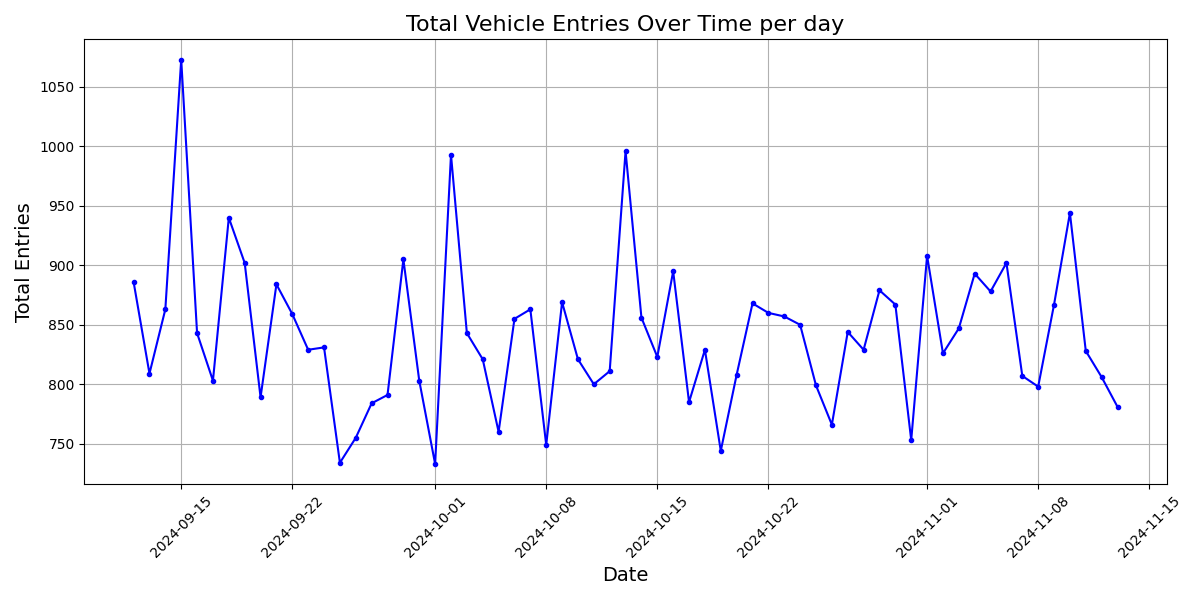
\includegraphics[width=0.8\textwidth]{plot10.png} % Adjust the width as needed
    \caption{Total vehicle entries per day(Time series in Part A)} % Add a caption if necessary
\end{figure}

\begin{figure}[h] % 'h' places the figure here, at the position in the text
    \centering % Center the figure
    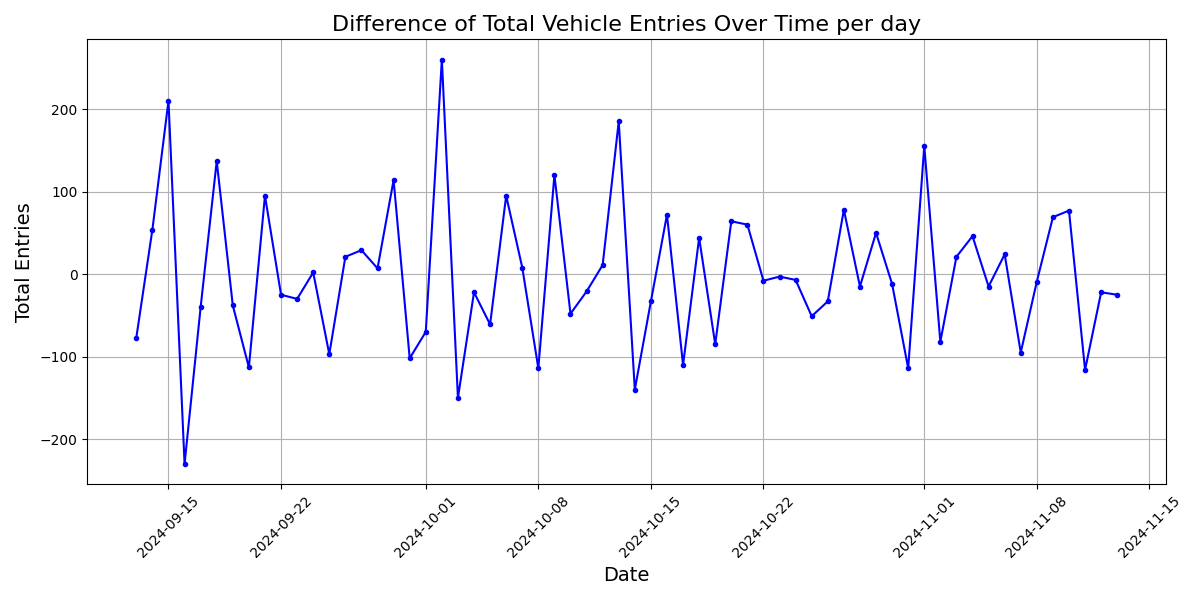
\includegraphics[width=0.8\textwidth]{plot11.png} % Adjust the width as needed
    \caption{Difference Series(d = 1) in Part A} % Add a caption if necessary
\end{figure}

\subsection{Part B}
\textbf{Check code in Q1b.ipynb} \newline
\newline 
\textbf{Answers: } \\
The values of \textbf{MASE(Mean absolute scaled error) and MAPE(Mean absolute percentage error)} for the test data(split from given data) are:
\begin{enumerate}
    \item MASE = 0.0921
    \item MAPE = 0.0062
\end{enumerate}
The predicted values of the average times in minutes spent in the mall by a vehicle entering on a particular day for the next 7 days is as follows:
\begin{enumerate}
    \item 14th November: 339.567819
    \item 15th November: 360.657282
    \item 16th November: 368.624311
    \item 17th November: 362.162941
    \item 18th November: 343.220077
    \item 19th November: 319.990320
    \item 20th November: 301.078917
\end{enumerate}

\begin{figure}[h] % 'h' places the figure here, at the position in the text
    \centering % Center the figure
    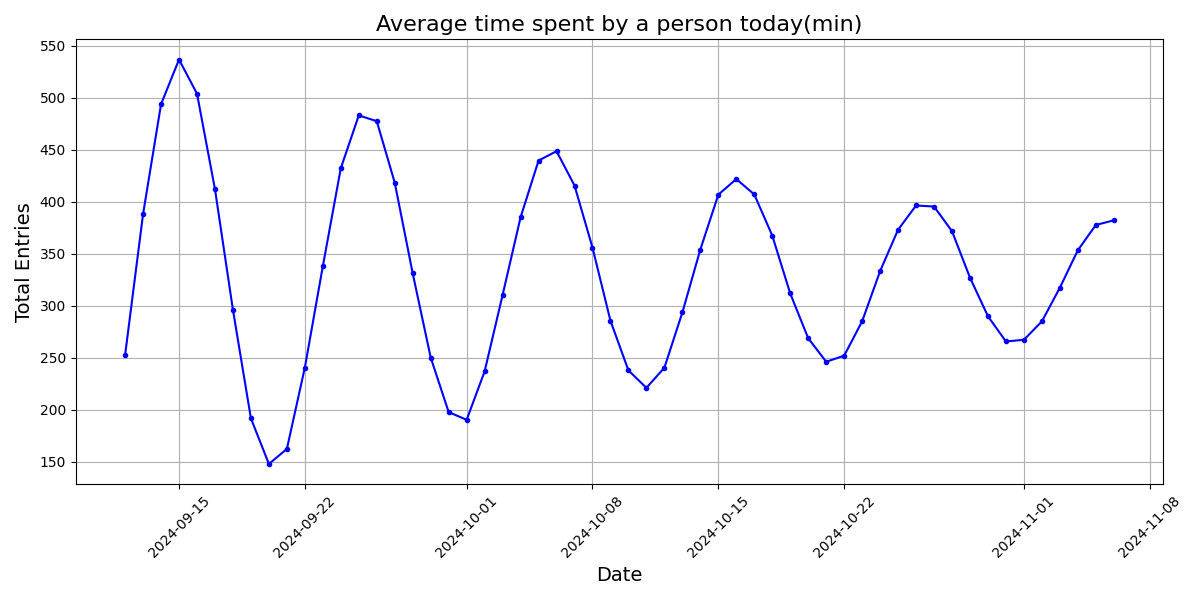
\includegraphics[width=0.8\textwidth]{plot20.png} % Adjust the width as needed
    \caption{Time Series in Part C(very smooth and has no trend)} % Add a caption if necessary
\end{figure}



\subsection{Part C}
\textbf{Check code in Q1c.ipynb} \newline
\newline 
\textbf{Answers: } \\
In this report, I have implemented two outlier smoothing routines to preprocess the data before feeding it into the model. These routines are:

\begin{enumerate}
    \item \textbf{Z-Score Outlier Smoothing:} This method calculates the Z-scores of the data points, which indicates how many standard deviations each point is from the mean. Any data point with an absolute Z-score greater than a specified threshold (commonly set to 3) is considered an outlier. These outliers are then replaced with the mean of the dataset to mitigate their influence on the analysis.
    
    \item \textbf{IQR Outlier Smoothing:} This method utilizes the interquartile range (IQR) to identify outliers. The IQR is computed as the difference between the third quartile (Q3) and the first quartile (Q1). Data points that lie below \( Q1 - 1.5 \times IQR \) or above \( Q3 + 1.5 \times IQR \) are classified as outliers. Similar to the Z-score method, these outliers are replaced with the mean of the dataset.
\end{enumerate}

The following table summarizes the Mean Absolute Percentage Error (MAPE) and Mean Absolute Scaled Error (MASE) for each part of the analysis, using the Z-score and IQR outlier smoothing methods.

\begin{table}[h]
    \centering
    \caption{Performance Metrics for Outlier Smoothing Methods}
    \begin{tabular}{@{}llcc@{}}
        \toprule
        \textbf{Part} & \textbf{Method} & \textbf{MAPE} & \textbf{MASE} \\ \midrule
        Part 1 & Z-Score & 0.0500 & 0.7442 \\ 
        Part 1 & IQR     & 0.0533 & 0.7911 \\ 
        Part 2 & Z-Score & 0.0062 & 0.0921 \\ 
        Part 2 & IQR     & 0.0062 & 0.0921 \\ \bottomrule
    \end{tabular}
\end{table}


%%%%%%%%%%%%%%%%%%%%%%%%%%%%%%%%%%%%%%%%%%%%%%%%%%%%%%%%%%%%%%

\section{Forecasting on a Real World Dataset
}
\subsection{Task 1}
\subsubsection{Part (a)}
\textbf{Code in Q2a.ipynb}\\
\\
\textbf{Hyperparameters are chosen : }
\begin{itemize}
    \item for p and q , the first significant spike drop observed in the \textbf{ACF} and \textbf{PACF} plots respectively is considered as optimal values
    \item As for d , \textbf{adfuller} function is used to determine optimal d value
\end{itemize}
\subsubsection{Part (b)}
\textbf{Code in Q2b.ipynb}\\
\\
\textbf{Best working prompt strategy : }\\
I have a time series dataset with 127 data points that represent monthly operational metrics for a major Indian airline from 2013. It includes information on the number of passengers traveled. The data follows an unknown model of time series. Based on this data, predict the next 12 values in the sequence and use the best model for the time series.\\
Please provide a list of 12 predicted values that could follow this series.\\
Here is the data: [\textbf{String of data generated using a python script}]\\
\\
\textbf{Evaluation of the prompt : }\\
\textbf{Data Frame : }7958524.0, 8050154.0, 8141784.0, 8233414.0, 8325044.0, 8416674.0, 8508304.0, 8599934.0, 8691564.0, 8783194.0, 8874824.0, 8966454.0\\
\textbf{MAPE of the dataframe predicted : }5.92
\subsubsection{Part (c)}
\textbf{Code in Q2c.ipynb}\\
\\
\textbf{Global Model used : }Neural Prophet\\
\textbf{Dataframe} : 7419019.5, 7914882.0, 8173941.0, 8574955.0, 8255045.5, 8246122.5, 8498941.0, 8273163.0, 8570758.0, 8351914.0, 8536465.0, 8747979.0\\
\textbf{MAPE of predicted data frame : }4.00
\subsection{Task 2}
\textbf{Solution: } \newline
\\
\textbf{Why MAPE may not be a good metric to evaluate the forecasts:}\\
\\
MAPE (Mean Absolute Percentage Error) measures forecast accuracy as a percentage error. While MAPE can be a useful metrics, it has notable limitations. Here are the primary reasons:
\\
\textbf{i. Sensitivity to Small Actual Values:}
\begin{itemize}
    \item MAPE calculates the percentage error by dividing the absolute error by the actual value for each data point.
    \item  If there are months with low passenger numbers (e.g., off-peak periods or months affected by events like COVID etc..) which results in low actual values, thus turns even small forecast errors to result in large percentage errors, which can distort the metric and make the forecast appear worse than it is.
\end{itemize}
\textbf{ii. Underrepresentation of Peak Demand:}
\begin{itemize}
    \item In fleet and workforce planning, airlines need to ensure they can handle peak demand periods, not just average demand.
    \item MAPE does not account for peak error directly and treats all errors equally, potentially underestimating the importance of errors during high-demand periods. An accurate understanding of peak periods is crucial since insufficient resources during these times can lead to significant operational disruptions and customer dissatisfaction.
\end{itemize}
\textbf{iii. Focus on Total Demand (Fleet Planning):}
\begin{itemize}
    \item Fleet requirements are typically dictated by total expected passenger numbers rather than percentage deviations. If the goal is to meet cumulative demand accurately, MAPE may not align well with this objective, as it emphasizes percentage accuracy rather than absolute volume.
\end{itemize}

\textbf{Suggested Alternative Metrics:}\\
\\
\textbf{i. Weighted Absolute Percentage Error (WAPE):}
\begin{itemize}
    \item WAPE is the sum of absolute errors divided by the sum of actual values, avoiding the problem of exaggerated errors at low values. This can give a more accurate picture of overall forecast performance without inflating errors in low-demand periods.
\end{itemize}
\textbf{ii. Root Mean Squared Error (RMSE):}
\begin{itemize}
    \item RMSE is effective for fleet planning because it emphasizes larger errors more heavily, providing a clearer picture of significant forecast deviations. By focusing on total volume error rather than percentage error, it better aligns with fleet planning needs, where the overall passenger count is essential.
\end{itemize}
\subsection{Task 3}
\textbf{Solution: } \newline
To compare whether there’s a structural break in the mean of this series before and after the COVID-19 period, we need a statistical test that can determine if there’s a significant change in mean from the pre-COVID period to the post-COVID period.\\
\textbf{Testing Method:}
\begin{itemize}
    \item Since we're looking at passenger counts specifically, we can perform a structural break test to see if there’s a significant difference in the mean of $\triangle$Y (first difference in monthly "Passengers Carried") across these periods.
\end{itemize}
\textbf{Suitable Test: Chow Test for Structural Break:}
\begin{itemize}
    \item \textbf{Purpose:} The Chow Test is a common test to detect structural breaks at a specific point in time in time-series data.
    \item \textbf{How it works:}
    \begin{itemize}
        \item The Chow test splits the time series at a given point—in this case, just before December 2019, with the post-COVID period starting after January 2022.
        \item The test compares the mean and other statistical properties of each segment, calculating an F-statistic to see if the model’s parameters (mean, in this case) are significantly different across the two time periods.
    \end{itemize}
    \item  \textbf{Assumptions:}
    \begin{itemize}
        \item The Chow Test assumes normally distributed errors, which fits well here as the first-differenced series is assumed stationary with known variance $\sigma^2$
    \end{itemize}
    \item \textbf{Interpretation:}
    \begin{itemize}
        \item If the test statistic is significant, it suggests a structural break, indicating that the mean of $\triangle$Y likely shifted post-COVID.
        \item  If the t-statistic is not significant, it suggests that the mean of monthly changes in passenger counts did not differ substantially, implying that the demand pattern may not have changed in terms of average month-to-month fluctuations.
    \end{itemize}
\end{itemize}
\textbf{Alternative: Two-Sample t-Test for Difference in Means:}
\begin{itemize}
    \item \textbf{Purpose: }If the primary objective is to test for a change in the mean of $\triangle Y$ across pre- and post-COVID periods, a Two-Sample t-Test for the difference in means can serve as a simpler alternative to the Chow Test.
    \item \textbf{How it works:}
    \begin{itemize}
        \item Calculate the mean of $\triangle Y$ for both periods.
        \item Use the t-test to compare the means. A significant t-statistic would indicate a difference in the average monthly change in passenger numbers, suggesting an impact from COVID-19
    \end{itemize}
    \item \textbf{Interpretation:}
    \begin{itemize}
        \item A significant t-statistic indicates that the average monthly change in passengers carried differs between the pre-COVID and post-COVID periods, supporting the hypothesis that COVID-19 structurally affected passenger demand.
    \end{itemize}
\end{itemize}
\textbf{Final thoughts:} the Chow test would be particularly suitable because it directly tests for a change in the relationship (mean in this case) before and after a specific point (pre-COVID and post-COVID periods)
%%%%%%%%%%%%%%%%%%%%%%%%%%%%%%%%%%%%%%%%%%%%%%%%%%%%%%%%%%%%%%

\end{document}